% Options for packages loaded elsewhere
\PassOptionsToPackage{unicode}{hyperref}
\PassOptionsToPackage{hyphens}{url}
\documentclass[
  british,
  11pt,
  a4paper,
]{article}
\usepackage{xcolor}
\usepackage[margin=25mm]{geometry}
\usepackage{amsmath,amssymb}
\setcounter{secnumdepth}{-\maxdimen} % remove section numbering
\usepackage{iftex}
\ifPDFTeX
  \usepackage[T1]{fontenc}
  \usepackage[utf8]{inputenc}
  \usepackage{textcomp} % provide euro and other symbols
\else % if luatex or xetex
  \usepackage{unicode-math} % this also loads fontspec
  \defaultfontfeatures{Scale=MatchLowercase}
  \defaultfontfeatures[\rmfamily]{Ligatures=TeX,Scale=1}
\fi
\usepackage{lmodern}
\ifPDFTeX\else
  % xetex/luatex font selection
\fi
% Use upquote if available, for straight quotes in verbatim environments
\IfFileExists{upquote.sty}{\usepackage{upquote}}{}
\IfFileExists{microtype.sty}{% use microtype if available
  \usepackage[]{microtype}
  \UseMicrotypeSet[protrusion]{basicmath} % disable protrusion for tt fonts
}{}
\makeatletter
\@ifundefined{KOMAClassName}{% if non-KOMA class
  \IfFileExists{parskip.sty}{%
    \usepackage{parskip}
  }{% else
    \setlength{\parindent}{0pt}
    \setlength{\parskip}{6pt plus 2pt minus 1pt}}
}{% if KOMA class
  \KOMAoptions{parskip=half}}
\makeatother
\usepackage{longtable,booktabs,array}
\newcounter{none} % for unnumbered tables
\usepackage{calc} % for calculating minipage widths
% Correct order of tables after \paragraph or \subparagraph
\usepackage{etoolbox}
\makeatletter
\patchcmd\longtable{\par}{\if@noskipsec\mbox{}\fi\par}{}{}
\makeatother
% Allow footnotes in longtable head/foot
\IfFileExists{footnotehyper.sty}{\usepackage{footnotehyper}}{\usepackage{footnote}}
\makesavenoteenv{longtable}
\usepackage{graphicx}
\makeatletter
\newsavebox\pandoc@box
\newcommand*\pandocbounded[1]{% scales image to fit in text height/width
  \sbox\pandoc@box{#1}%
  \Gscale@div\@tempa{\textheight}{\dimexpr\ht\pandoc@box+\dp\pandoc@box\relax}%
  \Gscale@div\@tempb{\linewidth}{\wd\pandoc@box}%
  \ifdim\@tempb\p@<\@tempa\p@\let\@tempa\@tempb\fi% select the smaller of both
  \ifdim\@tempa\p@<\p@\scalebox{\@tempa}{\usebox\pandoc@box}%
  \else\usebox{\pandoc@box}%
  \fi%
}
% Set default figure placement to htbp
\def\fps@figure{htbp}
\makeatother
\ifLuaTeX
\usepackage[bidi=basic,shorthands=off]{babel}
\else
\usepackage[bidi=default,shorthands=off]{babel}
\fi
\ifLuaTeX
  \usepackage{selnolig} % disable illegal ligatures
\fi
\setlength{\emergencystretch}{3em} % prevent overfull lines
\providecommand{\tightlist}{%
  \setlength{\itemsep}{0pt}\setlength{\parskip}{0pt}}
\usepackage{amsthm}
\usepackage{booktabs}
\usepackage{float}
\usepackage{needspace}
\floatplacement{figure}{H}
\setlength{\parskip}{4pt}
\usepackage{bookmark}
\IfFileExists{xurl.sty}{\usepackage{xurl}}{} % add URL line breaks if available
\urlstyle{same}
\hypersetup{
  pdftitle={Complementary disclosures in financial networks: accounting
geometry, prior-weighted uncertainty and bounded-error reports},
  pdfauthor={Anonymous},
  pdflang={en-GB},
  hidelinks,
  pdfcreator={LaTeX via pandoc}}

\title{Complementary disclosures in financial networks}
\usepackage{etoolbox}
\makeatletter
\providecommand{\subtitle}[1]{% add subtitle to \maketitle
  \apptocmd{\@title}{\par {\large #1 \par}}{}{}
}
\makeatother
\subtitle{Accounting geometry, prior-weighted uncertainty and
bounded-error reports}
\author{Anonymous}
\date{14 October 2026 · Version 2.0.0-candidate}

\begin{document}
\maketitle

\textbf{Version DOI:} \url{https://doi.org/10.5281/zenodo.23363516}

\textbf{Abstract.} Balance-sheet totals need not determine
outside-creditor losses after a financial network clears a known shock.
We study the residual range of this loss after exposure reports, rather
than the welfare consequences of disclosure. Two mechanisms must be
distinguished. On a coupled accounting simplex, an affine loss exhibits
all-or-nothing complementarity under a restricted report menu: one
interbank layer suffices for arbitrarily many jointly necessary reports.
For this affine class, standard linear-programming duality gives an
exact menu formula, an identification criterion and a bounded-error
extension. In a different, layered family, loss contains a product of
hidden allocation signs. We determine its uncertainty relative to the
shock and its dependence on the ratio of outside to interbank debt. For
independent priors used to weight full feasible fibres, we give the
exact expected width and a submodularity criterion valid also for
degenerate priors; cancellation of zero factors would give a false
criterion. We derive quantile widths, exhibit different optimal packages
under worst-case and expected-width criteria, and calculate
heterogeneous report-error effects. The treatment consolidates an
unpublished companion, identifies standard ingredients and
supplied-review contributions, and distinguishes written proofs, exact
finite checks, solver answers and historical records. The constructions
are synthetic; they imply neither prevalence in actual networks nor a
welfare-optimal disclosure policy.

\section{1. Question and contribution}\label{question-and-contribution}

A supervisor knows each bank's total interbank liabilities and assets,
outside debt and post-shock external assets, but not its bilateral
liabilities. Which reports identify outside-creditor loss after
proportional clearing, and which combinations are useful?

The question has three ingredients: an accounting-feasible set, a report
menu, and an uncertainty criterion. Omitting any can misidentify the
source of complementarity. Nonlinear loss is not needed for every
example: accounting identities can couple affine quantities, and a menu
can omit a directly informative report.

This paper is self-contained. Section 2 supplies clearing,
identification and selection. Section 3 treats the accounting-simplex
mechanism and gives an exact affine-menu characterisation. Section 4
studies the layered product mechanism. Sections 5 and 6 determine
prior-weighted and bounded-error widths. Section 7 separates
computational evidence by assurance level. Appendix A recovers the
earlier six-bank aggregate calculation.

The additions are quantitative and model-specific, not a new general
theory of informational complementarity or LP duality. Their strongest
significance limitation is that they concern deliberately constructed
networks and stipulated menus. Their useful output is exact diagnostics:
what a menu identifies, how much uncertainty remains, when the criterion
changes the optimal package, and how precision changes the answer.

\subsection{1.1 Relationship to earlier
work}\label{relationship-to-earlier-work}

The supplied unpublished working note, \emph{Optimal exposure disclosure
under clearing uncertainty} (Anonymous, 2026), already contains the pair
formulation, witness-cut selection, six-bank example, layered
construction at a particular parameter value, single-aggregate optimum
and robustness variants. It was not located as a public Evidence Press
release during this revision. We consolidate the required arguments
instead of directing readers to an unavailable published companion. The
original note is retained as a historical source, not a separately
verified current release.

{\def\LTcaptype{none} % do not increment counter
\begin{longtable}[]{@{}
  >{\raggedright\arraybackslash}p{(\linewidth - 2\tabcolsep) * \real{0.5000}}
  >{\raggedright\arraybackslash}p{(\linewidth - 2\tabcolsep) * \real{0.5000}}@{}}
\toprule\noalign{}
\begin{minipage}[b]{\linewidth}\raggedright
Ingredient
\end{minipage} & \begin{minipage}[b]{\linewidth}\raggedright
Relationship to prior material
\end{minipage} \\
\midrule\noalign{}
\endhead
\bottomrule\noalign{}
\endlastfoot
Proportional clearing and regularity & Eisenberg and Noe (2001);
specialised proof below \\
Pair width; midpoint error equal to half-width & Scalar optimal
recovery; supplied companion \\
Separating excessive-loss pairs & Test-cover/hitting-set formulation;
companion specialisation \\
Abstract high-order complementarity & XOR signals in Chen and Waggoner
(2016, §5.1) \\
Loss--shock bound & Consequence of loss conservation \\
One-layer affine construction & Supplied review; proved with menu
qualifications \\
Affine-simplex formula & Standard LP duality specialised to
disclosure \\
Layered family & Companion construction with general debt ratio \\
Prior and noise formulas & Quantitative analysis, corrected zero-factor
boundary and heterogeneous errors \\
\end{longtable}
}

Our objective differs from decision-theoretic value of information. Chen
and Waggoner (2016) analyse expected decision utility; our expected
criterion averages full accounting-feasible interval widths. Ahn, Chen
and Kim (2024) study partial information and worst-case shock
propagation, including several kinds of known bank and link information.
Their risk-quantification problem differs from choosing a finite report
package to minimise fixed-shock loss diameter on every fibre. Hu,
Mitchell and Tompaidis (2024) likewise consider robust financial
networks consistent with aggregate liabilities and assets, making their
framework a close benchmark rather than a generic adjacent citation. The
comparison here is limited to their publisher abstract, not a
theorem-level priority assessment. Feinstein et al.~(2018) analyse
clearing sensitivity to liability perturbations; our object is finite
report-consistent ambiguity, not a local derivative. These distinctions
delimit our contribution without claiming exhaustive exclusion of
earlier network-information work.

All monetary quantities use a common arbitrary unit. All networks
constructed here are synthetic.

\section{2. Clearing, feasible fibres and report
selection}\label{clearing-feasible-fibres-and-report-selection}

\subsection{2.1 Model and
well-posedness}\label{model-and-well-posedness}

There are \(n\ge1\) banks. The nominal liability \(L_{ij}\ge0\) goes
from bank \(i\) to bank \(j\), with \(L_{ii}=0\). Known totals satisfy
\[
\sum_jL_{ij}=r_i,\qquad\sum_iL_{ij}=a_j.
\] Each bank owes \(b_i>0\) outside and holds post-shock external assets
\(x_i\ge0\). Put \(\bar p_i=r_i+b_i\). The nonempty feasible set
\(\mathcal F\) consists of matrices with these totals, specified zeros
and any closed edge bounds. It is a compact polytope. Clearing satisfies
\[
p_i=\min\left\{\bar p_i,\ x_i+\sum_jL_{ji}\frac{p_j}{\bar p_j}\right\}.
\tag{1}
\] The right side is a contraction of the payment box in the \(1\)-norm
with constant at most \(\gamma=\max_i r_i/(r_i+b_i)<1\). It therefore
has a unique fixed point. The same constant works on \(\mathcal F\),
implying continuity in \(L\) by the usual fixed-point perturbation bound
with denominator \(1-\gamma\). For \(u_i=p_i/\bar p_i\),
outside-creditor loss is \[
\ell(L)=\sum_i b_i(1-u_i).
\tag{2}
\] The model excludes bankruptcy costs, fire sales and endogenous
reactions to disclosure.

The finite menu contains affine reports \(Q_q(L)\), \(q=1,\ldots,d\),
with costs \(c_q\ge0\). For selected reports \(S\) and feasible value
\(y\), define \[
\mathcal F(S,y)=\{L\in\mathcal F:Q_S(L)=y\},\qquad
w(S,y)=\max_{\mathcal F(S,y)}\ell-\min_{\mathcal F(S,y)}\ell .
\] The extrema exist on each nonempty compact fibre.

\subsection{2.2 Three uncertainty
criteria}\label{three-uncertainty-criteria}

The worst-case width is \[
R(S)=\sup_y w(S,y)
=\max_{\substack{L,M\in\mathcal F\\Q_S(L)=Q_S(M)}}[\ell(L)-\ell(M)].
\tag{3}
\] The pair-feasible set is compact and nonempty. On a scalar loss
interval, its midpoint minimises worst absolute estimation error, giving
error \(w/2\). Thus \(R/2\) is worst-case recovery error.

A prior \(\pi\) can weight likely reports: \[
W_\pi(S)=\mathbb E_\pi[w(S,Q_S(L))].
\tag{4}
\] \textbf{The fibre in (4) is the full accounting-feasible fibre, not
posterior support.} The prior supplies design weights while the
delivered interval protects against every accounting-feasible network.
This suits a prior used for planning but not trusted to exclude
alternatives. It differs from Bayesian posterior uncertainty; a
degenerate prior still does not remove unreported alternatives from
\(w\).

The \(1-\alpha\) quantile criterion is the least \(z\) with
\(\pi\{w(S,Q_S(L))\le z\}\ge1-\alpha\), for \(0<\alpha<1\).

Write \(G_V(S)=V(\varnothing)-V(S)\). This gain is monotone. Reports are
substitutes under \(V\) when \(G_V\) is submodular: a report's marginal
benefit cannot increase as the held set grows. A violation is
complementarity. A specified \(m\)-report menu is \emph{all-or-nothing}
when all proper subsets have zero gain and the full set has positive
gain. These properties concern the feasible set, menu and criterion
jointly.

\subsection{2.3 General lemmas}\label{general-lemmas}

\textbf{Lemma 1 (zero worst-case gain).} For compact \(\mathcal F\) and
continuous \(\ell,Q\), \(R(S)=R(\varnothing)\) exactly when a fibre of
\(Q_S\) contains a global maximiser and a global minimiser of \(\ell\).

\emph{Proof.} A maximal pair exists by (3). Its gap equals the global
range exactly when both global endpoints are attained. \(\square\)

\textbf{Lemma 2 (loss--shock bound).} If \(x^\circ\ge x\) and every bank
pays fully at \(x^\circ\), then for \(\sigma=\sum_i(x_i^\circ-x_i)\), \[
0\le\ell(L;x)\le\sigma.
\tag{5}
\]

\emph{Proof.} Let \(h_i=x_i+\sum_jL_{ji}u_j\) and
\(e_i=(h_i-\bar p_i)^+\). Cancelling interbank transfers gives
\(\ell=\sum_i b_i-\sum_i x_i+\sum_i e_i\). Payments, cash and equity are
monotone in \(x\). Since \(\ell(L;x^\circ)=0\),
\(\ell(L;x)=\sigma+\sum_i e_i(x)-\sum_i e_i(x^\circ)\le\sigma\).
Nonnegativity follows from \(u_i\le1\). \(\square\)

This useful computational bound follows from classical conservation,
explicitly discussed by Visentin, Battiston and D'Errico (2016, §3.2 and
Supplementary Information §2.2). Our constructions approach ratio one.
Inequality (5) alone does not establish universal nonattainment of
equality.

\textbf{Lemma 3 (product modules).} For disconnected modules with
product feasible set and module-local reports, \[
w(S,y)=\sum_k w_k(S_k,y_k),\quad
R(S)=\sum_k R_k(S_k),\quad
W_\pi(S)=\sum_kW_{\pi_k,k}(S_k).
\tag{6}
\] The last equality holds for \textbf{any joint prior} with marginals
\(\pi_k\).

\emph{Proof.} Fibres are products and losses sum. Maxima and minima
separate. Maximise over product report ranges for \(R\), and use
linearity of expectation for \(W\). No independence assumption on the
prior is needed. \(\square\)

\subsection{2.4 Exact selection as pair
separation}\label{exact-selection-as-pair-separation}

For tolerance \(\varepsilon\), each pair with
\(\ell(L)-\ell(M)>\varepsilon\) has distinguishing set
\(D(L,M)=\{q:Q_q(L)\ne Q_q(M)\}\). Formula (3) says
\(R(S)\le\varepsilon\) exactly when \(S\) hits every such set. This is a
scalar loss-tolerance specialisation of test cover.

A witness-cut algorithm solves a cost-minimising hitting-set master over
collected sets, then asks whether its selected reports admit another
excessive-loss pair. A verified pair adds a cut. An empty distinguishing
set proves menu infeasibility. UNSAT from a complete exact oracle
certifies optimality, since all previous cuts are necessary.

There are at most \(2^d\) distinguishing sets, and each newly found one
is not hit by the current solution. This proves termination with a
complete exact oracle, not a practical bound for nonlinear queries or
combinatorial selection. UNKNOWN is not infeasibility or optimality.
Real-algebraic SAT models need exact validation of their own; they are
not automatically rational certificates.

\section{3. Accounting geometry and the report
menu}\label{accounting-geometry-and-the-report-menu}

\subsection{3.1 One-layer affine
construction}\label{one-layer-affine-construction}

The following construction was suggested in the supplied review.

\textbf{Proposition 1 (affine loss, jointly necessary menu).} For every
\(m\ge1,b_s>0\), a \(2(m+1)\)-bank network with one interbank layer,
fixed totals and an \(m\)-report menu \(N\) satisfies \[
\ell(t)=b_s+t_0,\qquad R(S)=1\ (S\subsetneq N),\qquad R(N)=0.
\tag{7}
\] The shock is \(1+b_s\).

\emph{Proof.} Take \(k=m+1\) sources and sinks with a doubly stochastic
interbank block. Sources owe \(b_s\) outside and initially have assets
\(1+b_s\). Remove source 0's assets. Sinks owe one outside and no
interbank debt. Sink 0 has external assets zero; the others have one.

The shocked row is any \(t\in\Delta=\{t\ge0:\sum_{j=0}^m t_j=1\}\):
extend it by giving each other source row \((1-t)/m\). Unshocked sources
pay fully. Sink \(j\) receives \(1-t_j\); only sink 0 has outside
shortfall \(t_0\). The menu reports \(t_1,\ldots,t_m\), deliberately
omitting \(t_0\). The full menu identifies \(t_0\). For a proper subset
observed at zero, rows \(e_0,e_j\), for an unreported \(j\ge1\), agree
on the reports and differ in loss by one. Lemma 1 finishes the proof.
\(\square\)

The unresolved-loss ratio \(1/(1+b_s)\) approaches one at every fixed
order without interbank depth. One interbank layer does not mean one
defaulting bank layer: sink 0 may default as well as the shocked source.
Nonlinear loss or uncertain-recovery multiplication is not necessary on
the coupled feasible set. If \(t_0\) is available at the same cost,
however, one report identifies loss. The menu restriction is essential.

\subsection{3.2 Exact affine-simplex menu
formula}\label{exact-affine-simplex-menu-formula}

\textbf{Proposition 2.} Let \(t\in\Delta\subset\mathbb R^k\), loss
\(b+c^\mathsf Tt\), and selected affine reports with linear part \(A\).
Write \(\operatorname{osc}(v)=\max_i v_i-\min_i v_i\). Then \[
\begin{split}
R(A,c)&=\max_{\substack{t,u\in\Delta\\A(t-u)=0}}c^\mathsf T(t-u)\\
&=\min_\lambda\operatorname{osc}(c-A^\mathsf T\lambda)\\
&=2\min_{\lambda,\alpha}\|c-A^\mathsf T\lambda-\alpha\mathbf1\|_\infty .
\end{split}
\tag{8}
\] Under separate deterministic report-error bounds \(\eta_q\ge0\), \[
R_\eta(A,c)=\min_\lambda\left[
\operatorname{osc}(c-A^\mathsf T\lambda)+2\sum_q\eta_q|\lambda_q|
\right].
\tag{9}
\]

\emph{Proof.} Constants cancel. A multiplier \(\lambda\) for
\(A(t-u)=0\) gives the supremum
\(\max_{t,u\in\Delta}(c-A^\mathsf T\lambda)^\mathsf T(t-u)=\operatorname{osc}(c-A^\mathsf T\lambda)\).
Finite LP strong duality applies to this feasible bounded primal and
yields dual attainment. Centring at the midpoint of the extreme entries
proves the last equality.

With bounded errors, common observations exist exactly when
\(|A(t-u)|\le2\eta\). The two inequality multipliers have difference
\(\lambda\); the least penalty for a fixed difference is
\(2\sum_q\eta_q|\lambda_q|\), attained by positive and negative parts.
Duality gives (9), including zero tolerances and redundant rows.
\(\square\)

This is a specialisation of standard LP duality, as in Boyd and
Vandenberghe (2004, §§5.2.3--5.2.4), not new general duality. No rank
condition is needed. Rational primal and dual feasible solutions with
equal objective values provide exact certificates.

Consequently:

\begin{enumerate}
\def\labelenumi{\arabic{enumi}.}
\tightlist
\item
  \textbf{Identification:} \(R(A,c)=0\) iff
  \(c\in\operatorname{span}\{\mathbf1,\text{rows of }A\}\).
\item
  \textbf{Zero gain:} for extreme-index sets \(I_+,I_-\) of \(c\), and
  columns \(a_i\) of \(A\), \(R(A,c)=\operatorname{osc}(c)\) iff \[
  \operatorname{conv}\{a_i:i\in I_+\}\cap\operatorname{conv}\{a_i:i\in I_-\}\ne\varnothing.
  \tag{10}
  \]
\item
  \textbf{Coordinate reports:} for nonempty unreported set \(U\), \[
  w(S,t_S)=\left(1-\sum_{i\in S}t_i\right)\operatorname{osc}(c_U),\qquad
  R(S)=\operatorname{osc}(c_U).
  \tag{11}
  \] Empty or singleton unreported sets give zero width.
\end{enumerate}

For the first claim, zero gap on \(\ker A\cap\mathbf1^\perp\) implies
the span condition because the simplex difference set contains a
neighbourhood of zero in \(\mathbf1^\perp\); the converse is immediate.
A maximal-gap pair is supported on the two extreme coefficient sets,
giving (10). The residual simplex has mass \(1-\sum_{i\in S}t_i\),
giving (11), with worst case at \(t_S=0\).

This characterises widths for a fixed subset in the affine class. It
does not make arbitrary menu selection polynomial-time or generic
clearing affine.

Proposition 2 permits arbitrary affine coefficients and report matrices,
including asymmetric coefficients, redundant reports and alternative
menus containing the directly informative exposure. This supplies a
restricted-class robustness statement beyond the symmetric example. It
is not a theorem that complementarity survives every perturbation of
bank balance sheets: such perturbations may change both the feasible
domain and the clearing regime.

\subsection{3.3 Saturation and the product-domain
qualification}\label{saturation-and-the-product-domain-qualification}

A nonlinear one-layer example has \textbf{uniform} sink slack. Use
\(k\ge2\) sources and sinks with the same doubly stochastic block,
source outside debt \(b_s\), and complete shock to one source. Each sink
owes one outside and holds assets \(1/2\). Its shocked row gives \[
\ell(t)=b_s+\sum_{j=1}^k(t_j-\tfrac12)^+,\qquad
R(S)=
\begin{cases}\tfrac12,&|S|\le k-2,\\0,&|S|\ge k-1.\end{cases}
\tag{12}
\] With at least two unreported coordinates and observed values zero,
putting the remaining unit on one sink gives excess \(1/2\), while
spreading it equally gives zero. With \(k-1\) reports the last
coordinate is known. The full menu has a \((k-1)\)-of-\(k\) threshold;
any fixed \((k-1)\)-report submenu is all-or-nothing of order \(k-1\).

In contrast, for a product box, separable loss \(\sum_jg_j(t_j)\), and
coordinate reports, \[
R(S)=\sum_{j\notin S}\operatorname{osc}(g_j),
\tag{13}
\] so gain is modular. All three assumptions matter: Proposition 1 has
affine loss but a simplex, not a product box. Feasible geometry, menu
restrictions and nonlinear transmission are distinct mechanisms.

\section{4. The layered product
mechanism}\label{the-layered-product-mechanism}

\subsection{4.1 Construction and debt
ratio}\label{construction-and-debt-ratio}

Fix \(m\ge1,\beta>0,b_0>0\). Layer \(j\), \(j=0,\ldots,m\), has banks
\(2j,2j+1\). Between successive layers the liability block is \[
T(t_j)=\begin{pmatrix}t_j&1-t_j\\1-t_j&t_j\end{pmatrix},
\qquad t_j\in[0,1],\quad j=1,\ldots,m.
\] There are no other interbank liabilities. Sources owe \(b_0\)
outside, intermediates owe \(\beta\) outside, and final banks owe one
outside. Before the shock, external assets are \(1+b_0\) at each source,
\(\beta\) at each intermediate, and \((0,1)\) at the final pair. All pay
fully. Removing bank 0's assets gives shock \(\sigma=1+b_0\).

Each interlayer block has unit row and column sums independent of its
switch. Sources have interbank column sum zero and row sum one;
intermediates have both one; final banks have row sum zero and column
sum one. Totals are fixed but not all one at the boundary. Reports are
\(t_j=L_{2(j-1),2j}\). The parameter \(\beta\) is the
\textbf{outside-to-interbank debt ratio}, not the outside share; that
share is \(\beta/(1+\beta)\).

\begin{figure}
\centering
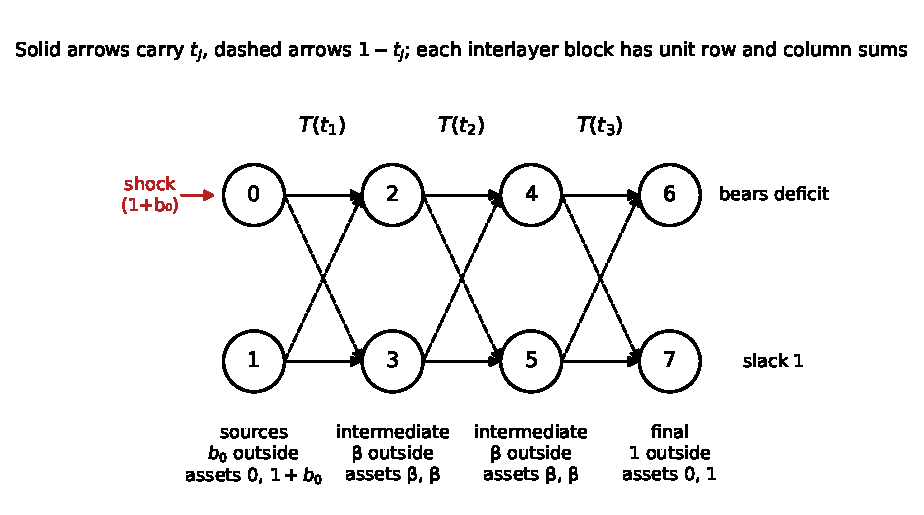
\includegraphics[width=1\linewidth,height=\textheight,keepaspectratio,alt={The layered family at m=3. Each interlayer block has unit row and column sums; source and final-layer boundary totals differ as described in the text. Each intermediate layer transfers the fraction \textbackslash beta/(1+\textbackslash beta) of its incoming deficit to outside creditors. Uncertain residual allocation determines final-layer loss.}]{figure_layered.pdf}
\caption{The layered family at \(m=3\). Each interlayer block has unit
row and column sums; source and final-layer boundary totals differ as
described in the text. Each intermediate layer transfers the fraction
\(\beta/(1+\beta)\) of its incoming deficit to outside creditors.
Uncertain residual allocation determines final-layer loss.}
\end{figure}

\subsection{4.2 Exact loss and widths}\label{exact-loss-and-widths}

\textbf{Theorem A (layered magnitude).} Put \(c=(1+\beta)^{1-m}\). For
every \(t\in[0,1]^m\), \[
\ell_m(t)=1+b_0-\frac c2\left(1-\prod_{j=1}^m(2t_j-1)\right).
\tag{14}
\] For \(S\subsetneq N=\{1,\ldots,m\}\), \[
w(S,t_S)=c\prod_{j\in S}|2t_j-1|,\qquad R(S)=c,
\tag{15}
\] whereas \(R(N)=0\). If switches are restricted to \([a,1-a]\),
\(0\le a<1/2\), and \(h=1-2a\), then for proper \(S\), \[
w(S,t_S)=c\,h^{m-|S|}\prod_{j\in S}|2t_j-1|,
\qquad R(S)=c h^m,
\tag{16}
\] with zero width after full disclosure.

\emph{Proof.} Bank 0 pays nothing and bank 1 pays fully. The deficit
entering layer 1 is \(d_1=T(t_1)^\mathsf T(1,0)^\mathsf T\). An
intermediate bank receiving deficit \(s\in[0,1]\) has recovery
\(1-s/(1+\beta)\), outside loss \(\beta s/(1+\beta)\), and transmits
interbank deficit \(s/(1+\beta)\). Thus \[
d_{j+1}=(1+\beta)^{-1}T(t_{j+1})^\mathsf T d_j,\qquad
\|d_j\|_1=(1+\beta)^{1-j}.
\] These bounds keep banks in the stated linear regime. The common
eigenvectors of \(T(t)\) are \((1,1)^\mathsf T,(1,-1)^\mathsf T\), with
eigenvalues \(1,2t-1\). Hence \[
d_m=\frac c2\left[(1,1)^\mathsf T+
\prod_j(2t_j-1)(1,-1)^\mathsf T\right].
\] Intermediate outside losses sum to \(1-c\). The first final bank
loses the first component of \(d_m\), and the second final bank's unit
slack absorbs its deficit. Adding source outside loss \(b_0\) gives
(14).

For proper \(S\), the free-sign product ranges over \([-1,1]\), proving
(15). On the restricted box it ranges over \([-h^{m-|S|},h^{m-|S|}]\),
proving (16). Endpoint choices attain the maxima. \(\square\)

The unresolved-loss ratio is \[
\frac{R(\varnothing)}{\sigma}
=\frac{(1+\beta)^{1-m}}{1+b_0}.
\tag{17}
\] For \(b_0=\beta\) it is \((1+\beta)^{-m}\), exponentially decreasing
in \(m\) at fixed positive \(\beta\). For each fixed \(m\) and
\(\varepsilon\in(0,1)\), choosing \[
0<\beta\le(1-\varepsilon)^{-1/m}-1
\] makes the ratio at least \(1-\varepsilon\). Maintaining that
guarantee as \(m\) grows requires \(\beta\) of order \(1/m\), not a
fixed positive value. Ratios approach one in this family but do not
attain it at its positive parameters. Proposition 1 reaches the same
supremum without depth.

{\def\LTcaptype{none} % do not increment counter
\begin{longtable}[]{@{}rrrr@{}}
\toprule\noalign{}
\(m\) & \(\beta=1\) & \(\beta=1/10\) & \(\beta=1/100\) \\
\midrule\noalign{}
\endhead
\bottomrule\noalign{}
\endlastfoot
1 & 0.500 & 0.909 & 0.990 \\
2 & 0.250 & 0.826 & 0.980 \\
4 & 0.063 & 0.683 & 0.961 \\
6 & 0.016 & 0.564 & 0.942 \\
10 & 0.001 & 0.386 & 0.905 \\
\end{longtable}
}

\emph{Table 1. Formula \((1+\beta)^{-m}\), rounded to three decimals,
with \(b_0=\beta\). These are mathematical evaluations, not empirical
estimates.}

\section{5. Priors weight fibres; they do not redefine
them}\label{priors-weight-fibres-they-do-not-redefine-them}

\subsection{5.1 Expected widths and the zero-factor
boundary}\label{expected-widths-and-the-zero-factor-boundary}

\textbf{Theorem B (corrected prior criterion).} Let the switches be
independent under \(\pi\), with
\(\kappa_j=\mathbb E_\pi|2t_j-1|\in[0,1]\). Then \[
W_\pi(S)=c\prod_{j\in S}\kappa_j\quad(S\subsetneq N),\qquad W_\pi(N)=0.
\tag{18}
\] For \(m\ge2\), expected-width gain is submodular exactly when, for
each distinct \(i,j\), \[
\left(\prod_{k\notin\{i,j\}}\kappa_k\right)(1-\kappa_i-\kappa_j)\ge0.
\tag{19}
\] Equivalently, either some \(\kappa_j=0\), or every pair satisfies
\(\kappa_i+\kappa_j\le1\). For \(m=1\) submodularity is automatic.

\emph{Proof.} Formula (18) follows from (15) and independence. For
distinct \(i,j\notin S\), when \(Sij=S\cup\{i,j\}\) is proper, the
elementary submodularity difference is \[
G(Si)+G(Sj)-G(S)-G(Sij)
=c\prod_{k\in S}\kappa_k(1-\kappa_i)(1-\kappa_j)\ge0.
\] When \(S\cup\{i,j\}=N\), the difference is the left side of (19)
times \(c\). These elementary inequalities are necessary and sufficient,
because general diminishing-return inequalities follow by adjoining one
element at a time. This proves the condition without cancelling any
factor.

If all factors are positive, cancel them to obtain the pair-sum
conditions. If \(\kappa_z=0\), a pair not containing \(z\) has zero
prefactor; a pair containing \(z\) has nonnegative final factor. Hence
every zero-containing vector satisfies (19). \(\square\)

At \((\kappa_1,\kappa_2,\kappa_3)=(0,3/4,3/4)\), gain is submodular
despite a pair sum \(3/2\). Strict final-two-report complementarity
requires both \(\kappa_i+\kappa_j>1\) and
\(\prod_{k\notin\{i,j\}}\kappa_k>0\).

Uniform switches have \(\kappa=1/2\), giving equality in completion
inequalities, but not necessarily modularity when \(m>2\). Other
examples are \(3/8\) for Beta\((2,2)\), \(9/16\) for Beta\((1,3)\), and
\(2/\pi\) for Beta\((1/2,1/2)\). Endpoint-supported priors have
\(\kappa=1\) and yield the worst-case width set function. This concerns
(4), not equality of posterior and worst-case uncertainty.

For a proper unit-cost budget \(k<m\), the \(k\) smallest \(\kappa_j\)
minimise (18). Greedy expected-width selection is therefore optimal in
this family, with harmless ties after a zero is selected; no such
general guarantee is claimed for clearing networks.

\subsection{5.2 Quantile corollary}\label{quantile-corollary}

\textbf{Corollary C.} For independent uniform switches and \(1\le n<m\)
observed reports, \[
q_n(\alpha)=c\exp[-\gamma_n(\alpha)],
\tag{20}
\] where \(q_n\) is the \(1-\alpha\) quantile of realised width and
\(\gamma_n\) is the \(\alpha\)-quantile of Gamma\((n,1)\). With no
reports \(q_0=c\); with all reports \(q_m=0\).

\emph{Proof.} The \(U_j=|2t_j-1|\) are independent uniform variables.
Thus \(-\log\prod_{j=1}^nU_j\) is Gamma\((n,1)\), and
\(c\prod U_j>q_n(\alpha)\) has probability \(\alpha\). \(\square\)

This uses the standard product-of-uniforms transformation. After six of
at least seven reports the 95th percentile is about \(0.073c\): the
realised width exceeds this threshold with probability 5\%. It is not a
5\% probability of a false reported interval. Each realised full-fibre
interval retains its accounting guarantee.

\subsection{5.3 Exact optima can depend on the
criterion}\label{exact-optima-can-depend-on-the-criterion}

\textbf{Proposition 3.} Take a six-bank core with \(m=2,\beta=b_0=1\),
reports \(x,y\), and two disconnected four-bank single-switch modules
scaled to widths \(7/20,1/10\), reports \(z_1,z_2\). With unit costs and
budget two, the unique minimax optimum is \(\{x,y\}\), width \(9/20\).
Under independent uniform switch priors, expected-width optima are
\textbf{both} \(\{x,z_1\}\) and \(\{y,z_1\}\), width \(7/20\).

\emph{Proof.} Lemma 3 and Theorem B give all possibilities:

{\def\LTcaptype{none} % do not increment counter
\begin{longtable}[]{@{}lrr@{}}
\toprule\noalign{}
Package & Worst-case width & Expected width \\
\midrule\noalign{}
\endhead
\bottomrule\noalign{}
\endlastfoot
\(\{x,y\}\) & \(9/20\) & \(9/20\) \\
\(\{z_1,z_2\}\) & \(1/2\) & \(1/2\) \\
\(\{x,z_1\}\) or \(\{y,z_1\}\) & \(3/5\) & \(7/20\) \\
\(\{x,z_2\}\) or \(\{y,z_2\}\) & \(17/20\) & \(3/5\) \\
\end{longtable}
}

Monotonicity excludes improvement by a smaller package. \(\square\)

The worst case gives no credit for one core report; expectation credits
its typical fibre reduction. Neither criterion is universally
preferable.

\section{6. Bounded reporting error}\label{bounded-reporting-error}

Each reported value has arbitrary error bounded by \(\eta_q\ge0\). Two
networks share a possible observation exactly when \[
|Q_q(L)-Q_q(M)|\le2\eta_q\qquad(q\in S),
\tag{21}
\] because their error intervals intersect. Formula (3) with this
constraint gives noisy width. It models bounded additive uncertainty,
not fixed rounding bins or random measurement errors.

For layered switches put \(\delta_j=\min(4\eta_j,2)\),
\(D=\max_j\delta_j\). The factor four converts pair differences in
\(t_j\) into differences of \(2t_j-1\).

\textbf{Lemma 4 (heterogeneous product gap).} For \(m\ge1\),
\(\delta_j\in[0,2]\), and \(a,a'\in[-1,1]^m\) satisfying
\(|a_j-a'_j|\le\delta_j\), the maximal product gap is \[
F(\delta)=
\begin{cases}
1-\prod_j(1-\delta_j),&D\le1,\\
D,&D\ge1.
\end{cases}
\tag{22}
\] The two expressions agree at \(D=1\).

\emph{Proof.} If \(D\le1\) and a coordinate pair has opposite signs, the
gap is at most \(|a_j|+|a'_j|\le\delta_j\le1-\prod_i(1-\delta_i)\).
Otherwise take each pair's absolute values, preserving the modulus of
the product gap, and suppose \(\prod a\ge\prod a'\). For fixed \(a\),
the least admissible \(a'_j\) is \((a_j-\delta_j)^+\). If some
\(a_j<\delta_j\), the gap is at most \(a_j\le D\), bounded by the stated
expression. Otherwise \(\prod_j a_j-\prod_j(a_j-\delta_j)\) is
nondecreasing in every coordinate, since its partial derivatives are
nonnegative. Its maximum occurs at \(a=\mathbf1\), attained with
\(a'_j=1-\delta_j\).

For \(D\ge1\), common signs in every coordinate give products of common
sign and gap at most one. Otherwise an opposite-sign pair bounds the gap
by \(\delta_j\le D\). Set \(a=\mathbf1\), change one coordinate of
\(a'\) to \(1-D\) where \(\delta_j=D\), and leave the rest one. This
attains \(D\). \(\square\)

\textbf{Theorem D.} With \(c=(1+\beta)^{1-m}\), \[
R_\eta(N)=\frac c2F(\delta),\qquad R_\eta(S)=c\quad(S\subsetneq N).
\tag{23}
\]

\emph{Proof.} Formula (14) makes the loss gap \(c/2\) times the product
gap. Constraints (21) are those of Lemma 4; clipping at two changes no
feasible pair. A proper subset already has a noiseless pair attaining
global width \(c\), which no noisy pair exceeds. \(\square\)

Equal errors \(0\le\eta\le1/4\) recover \[
R_\eta(N)=\frac c2[1-(1-4\eta)^m].
\tag{24}
\] If every \(\eta_j\le1/4\), the residual fraction is \[
\frac{R_\eta(N)}c=\frac12[1-\prod_j(1-4\eta_j)]\le2\sum_j\eta_j.
\] For fixed \(m\), it is asymptotic to \(2\sum_j\eta_j\) as the nonzero
error vector tends to zero. This is not the coarse-error formula. If
some \(\eta_j\ge1/2\), full disclosure leaves width \(c\).

At \(m=2,\beta=1,\eta=1/100\), the residual is \(49/2500=0.0196\), or
\(0.0392\) of initial width. Eight reports each with \(\eta=1/1000\)
leave about \(0.0158\) of initial width. These are model calculations,
not practical reporting recommendations.

\section{7. Computational evidence and reproducibility
boundaries}\label{computational-evidence-and-reproducibility-boundaries}

Written proofs establish continuum statements. Finite arithmetic checks
test implementations and selected consequences; solver checks test
formulations without supplying the closed form. Neither constitutes
proof-assistant verification.

\subsection{7.1 Supplied audit and current
replay}\label{supplied-audit-and-current-replay}

A current producer-side replay of the supplied pure-arithmetic audit
passed 1,740 layered clearing checks, 1,260 endpoint-width checks, 336
realised-width checks, 239 saturation checks, 775 prior-parameter
vectors, 12 noisy configurations and 400 cyclic loss--shock cases. The
prior grid contains 302 counterexamples to the original
zero-cancellation criterion; the corrected condition passes. These are
finite tests, not complete parameter coverage. This supplied-audit
replay used normal Python mode.

The review separately supplies 25 quantile comparisons and a one-layer
script recording 441 exact clearing evaluations, 360 endpoint checks and
12 full-matrix solver queries. These supplied counts are distinct from
current pure-arithmetic replay counts. ``Review'' identifies supplied
materials, not verified external peer review, human reviewer identity or
independent reproduction.

A separate original release checker,
\textbf{code/verify\_extensions.py}, passed in normal and optimised
Python modes. It checks 70 exact affine primal/dual certificates, the
775 prior vectors, 155 heterogeneous-error configurations across 11,154
product-polytope vertices, 375 one-layer rational clearing cases and 78
proper-menu endpoint pairs. Seven negative controls reject malformed
certificates or invalid error-domain reasoning. Receipts are
\textbf{logs/pypi-extensions-normal.json} and
\textbf{logs/pypi-extensions-optimized.json}. These are finite exact
checks supporting, not replacing, the proofs.

\subsection{7.2 Historical random-network
study}\label{historical-random-network-study}

The original package explores 32 three-report feed-forward instances,
six four-report instances and six cyclic instances. Its records report
24 completed and eight unresolved three-report cases, four completed
four-report cases, and one completed cyclic case. The old solver
handling did not uniformly retain separately replayable exact rational
witnesses for every SAT result. Those counts and brackets are
\textbf{historical records}, not a freshly certified prevalence sample.

The three-report generator requests \(2n+2\) edges but is capped by
\(n(n-1)/2\); five-bank runs have ten actual edges, not twelve. A
bracket with lower endpoint zero does not prove zero width. The legacy
selection target was half the \emph{upper endpoint} of the initial
bracket, not half its true width; at tolerance \(\sigma/64\) this can
overshoot by \(\sigma/128\). Longest-query timings omit some selection
work, and wall times can include unsuccessful calls.
Completion-conditioned results are not population frequencies; small
unmatched samples do not establish cycles as the cause of solver
difficulty. The original headline prevalence and timing claims are
therefore not repeated as current conclusions.

\subsection{7.3 Fresh retained-witness
study}\label{fresh-retained-witness-study}

A fresh run reused the 44 historical \emph{input specifications}, not
their answers, with the repaired code, Z3 5.1.0, two workers, a
40-second timeout per solver call and bracket tolerance \(\sigma/64\).
Every instance and every query was retained in
\textbf{results/fresh-full/}. The aggregation in
\textbf{results/fresh-study-aggregation.json} gives:

\Needspace{18\baselineskip}

{\def\LTcaptype{none} % do not increment counter
\begin{longtable}[]{@{}lrrrr@{}}
\toprule\noalign{}
Input group & Inputs & Width-complete & Unresolved & Zero shock \\
\midrule\noalign{}
\endhead
\bottomrule\noalign{}
\endlastfoot
DAG, 5 or 6 banks, 3 reports & 16 & 14 & 2 & 0 \\
DAG, 8 or 10 banks, 3 reports & 16 & 10 & 5 & 1 \\
DAG, 6 banks, 4 reports & 6 & 4 & 2 & 0 \\
Cyclic, 4--6 banks, 3 reports & 6 & 1 & 5 & 0 \\
Total & 44 & 29 & 14 & 1 \\
\end{longtable}
}

\emph{Table 2. Fresh finite run. Width-complete means every requested
width bracket completed, not that all conceivable questions about that
instance were resolved. The zero-shock instance was identified
separately and required no solver queries. All eight five-bank DAG
inputs have ten actual allowed edges, although twelve were requested.}

Among the 29 width-complete instances, 28 have a strictly positive
witnessed initial width. The remaining instance has a separate UNSAT
answer to the strictly-positive-gap query; its zero-width classification
does not rest on a zero lower bracket. Four of the 28 positive-width
instances have bracket-certified violations of submodularity. These
observations are conditional on these inputs, timeout and completion
rule; neither the proportion nor its change from the historical run
estimates population prevalence.

Selection was attempted only for those 28 positive-width instances, with
the implemented target \(R_{0,\mathrm{upper}}/2\). Seven returned an
optimal package and 21 returned that no subset of the supplied menu
meets this target; none of these selection attempts remained unresolved.
The target can exceed half the true initial width by at most
\(\sigma/128\). This is menu infeasibility, not inconsistency of the
underlying network constraints.

Accounting-redundancy queries screened 91 reports across the 29
width-complete instances: 24 were fixed by the accounting constraints,
67 had exact witnessed variation, and none of these screens was
unresolved. Of 65 reports whose singleton gain was certified at most
\(\sigma/64\), 24 were accounting-fixed and 41 were accounting-variable.
The other 26 reports were variable but were not certified negligible;
this alone is not a positive-gain certificate. The screen does
\textbf{not} establish that a variable report affects loss, lies in the
loss-relevant shocked component, or becomes useful only jointly. Those
stronger distinctions remain outside this finite audit. In particular,
negligible singleton gain is not automatically evidence of
complementarity.

The 1,878 retained queries contain 657 exactly checked rational
witnesses, 1,207 solver UNSAT answers and 14 UNKNOWN answers; no
solver-only algebraic SAT arose in this run. Replaying all retained
rational witnesses and metadata checks passed in normal and optimised
Python modes, with receipts \textbf{logs/assurance-final-normal.json}
and \textbf{logs/assurance-final-optimized.json}. These replays do not
turn UNSAT answers into independently checked unsatisfiability
certificates. The verifier also exercises the algebraic-SAT and UNKNOWN
branches through explicit controls.

The two-worker elapsed time was 3,006.9 seconds (50 minutes 6.9
seconds), measured between the run's UTC start and finish. The longest
solver call was 40.6744 seconds; the longest query wall time, including
extraction and checking overhead, was 40.6864 seconds. Both maxima
include all retained stages, including selection and redundancy, and the
elapsed time includes unresolved calls. A requested solver timeout is
not an exact wall-clock cap. The unmatched groups and small cyclic
sample do not identify a causal runtime effect of cycles.

\subsection{7.4 Certificate semantics}\label{certificate-semantics}

For a query asking whether a gap exceeds a threshold, an exact validated
witness supplies an attained lower bound. UNSAT supplies a
solver-relative upper bound. SAT without a separately checked exact
witness is solver-only evidence and does not advance a witness-certified
lower bound. UNKNOWN preserves the bracket and is not infeasibility,
including at initial feasibility or selection.

Reusable witnesses record both matrices, recoveries, gap, selected
reports and equality or error constraints, instance data, threshold,
solver version and checksums. Algebraic models require exact algebraic
validation or an explicit unverified label. In the affine-simplex class,
rational primal and dual feasible solutions of equal objective certify a
width without nonlinear solving.

Final release receipts identify fresh checks and hashes. Historical
outputs remain separately labelled; parsing an old JSON does not promote
it to verified evidence. Reproduction is producer-side unless
independent external reproduction is specifically documented.

\section{8. Interpretation and limits}\label{interpretation-and-limits}

There is no unconditional ``value of a report.'' Changing the
uncertainty criterion can change an optimal package. Our prior-weighted
criterion retains full feasible fibres; posterior-support widths answer
a different question.

On a simplex, restricted menus make affine measurements jointly
sufficient. On a product domain, layered loss creates a multiplicative
interaction with calculable magnitude and precision sensitivity.
Saturation supplies another example. These do not exhaust clearing
mechanisms. Proposition 2 completely characterises width only in its
stated affine-simplex class.

Depth is not necessary for arbitrary-order complementarity. Nor is the
saturation example's half-deficit range a universal one-layer bound:
Proposition 1 disproves that interpretation. Open questions concern
realistic accounting constraints and menus, collection versus
transmission costs, and scalable certified bounds for nonlinear
clearing.

These are identification results, not welfare or actual
financial-stability conclusions. No actual bank data are analysed. This
is an unrefereed candidate with written arguments and finite checks at
stated scopes, not a formally verified theorem collection or
independently reproduced empirical study.

\section{Appendix A. The six-bank aggregate
calculation}\label{appendix-a.-the-six-bank-aggregate-calculation}

This content is inherited from the supplied companion. Set
\(m=2,b_0=\beta=1\), with switches \(x,y\). Then \[
\ell(x,y)=\frac74+\frac14(2x-1)(2y-1).
\] Each individual exposure has zero guaranteed gain; both identify
loss. A different one-report menu halves initial width. For \(s=x+y\),
\[
w(s)=\frac14\min(s,2-s)^2,\qquad0\le s\le2,
\] with worst case \(1/4\), versus initial \(1/2\). On \(0\le s\le1\),
\(xy\) ranges from zero to \(s^2/4\); reflection gives the other half.

This is optimal among single nonconstant affine scalar reports on the
square. Reflecting either coordinate preserves absolute loss gaps;
exchanging coordinates is a symmetry. A report using both can be
normalised to \(x+t y\), \(0<t\le1\). On its fibre \(x+t y=1\), the
variable part of twice the loss, up to sign, is \[
g_t(y)=(1+t)y-2t y^2,\qquad0\le y\le1.
\] Its minimum is zero. For \(t\le1/3\), its maximum is \(1-t\), giving
width at least \(1/3\). For \(t\ge1/3\), its maximum is
\((1+t)^2/(8t)\), giving width at least \((1+t)^2/(16t)\ge1/4\). A
report using only one coordinate leaves width \(1/2\). Hence \(x+y\) is
optimal. This assumes exact real reports and ignores aggregate
collection costs.

The companion's greedy failure adds a disconnected one-report module of
width \(0<\delta<1/2\) to this core with budget two. Greedy worst-case
gain takes the decoy first; one remaining report cannot complete the
core, so gain is only \(\delta\). The optimal core pair gains \(1/2\).
The ratio \(2\delta\) tends to zero. This concerns gain under that
greedy rule, not residual-width approximation or all algorithms.

\section{Provenance and availability}\label{provenance-and-availability}

The canonical source is this Markdown manuscript. The companion is
retained as the historical unpublished file
\textbf{provenance/companion-2026-10-13.md}; its exact original hash and
input identity are recorded in the package's provenance record.
Retention does not endorse every historical computational claim.

The revision and checks are producer-coordinated. The one-layer
construction is credited to the supplied review. No human contribution,
external peer-review status or exhaustive novelty determination is
inferred from those materials. The examples contain no participants or
identifiable institution data. Code and verification records accompany
the release at stated scopes.

\begingroup\small

\section{References}\label{references}

Ahn, D., Chen, N., \& Kim, K.-K. (2024). Robust risk quantification via
shock propagation in financial networks. \emph{Operations Research,
72}(1), 1--18. \url{https://doi.org/10.1287/opre.2020.0722}

Anonymous. (2026, October 13). \emph{Optimal exposure disclosure under
clearing uncertainty} {[}Unpublished working note supplied with the
candidate; original archived in the release package{]}.

Boyd, S., \& Vandenberghe, L. (2004). \emph{Convex optimization}.
Cambridge University Press.
\url{https://web.stanford.edu/~boyd/cvxbook/}

Chen, Y., \& Waggoner, B. (2016). Informational substitutes. In
\emph{Proceedings of the 57th Annual IEEE Symposium on Foundations of
Computer Science} (pp.~239--247). Full version: arXiv:1703.08636v1.
\url{https://arxiv.org/abs/1703.08636}

De Bontridder, K. M. J., Halldórsson, B. V., Halldórsson, M. M.,
Hurkens, C. A. J., Lenstra, J. K., Ravi, R., \& Stougie, L. (2003).
Approximation algorithms for the test cover problem. \emph{Mathematical
Programming, 98}, 477--491.
\url{https://doi.org/10.1007/s10107-003-0414-6}

Eisenberg, L., \& Noe, T. H. (2001). Systemic risk in financial systems.
\emph{Management Science, 47}(2), 236--249.
\url{https://doi.org/10.1287/mnsc.47.2.236.9835}

Feinstein, Z., Pang, W., Rudloff, B., Schaanning, E., Sturm, S., \&
Wildman, M. (2018). Sensitivity of the Eisenberg--Noe clearing vector to
individual interbank liabilities. \emph{SIAM Journal on Financial
Mathematics, 9}(4), 1286--1325. \url{https://doi.org/10.1137/18M1171060}

Hu, F., Mitchell, D., \& Tompaidis, S. (2024). Robust financial
networks. \emph{Operations Research, 72}(5), 1827--1842.
\url{https://doi.org/10.1287/opre.2022.0272}

Micchelli, C. A., \& Rivlin, T. J. (1977). A survey of optimal recovery.
In C. A. Micchelli \& T. J. Rivlin (Eds.), \emph{Optimal estimation in
approximation theory} (pp.~1--54). Springer.
\url{https://doi.org/10.1007/978-1-4684-2388-4_1}

Visentin, G., Battiston, S., \& D'Errico, M. (2016). \emph{Rethinking
financial contagion} {[}Preprint{]}. arXiv:1608.07831v1.
\url{https://arxiv.org/abs/1608.07831}

de Moura, L., \& Bjørner, N. (2008). Z3: An efficient SMT solver. In
\emph{Tools and algorithms for the construction and analysis of systems
(TACAS 2008)} (pp.~337--340).
\url{https://doi.org/10.1007/978-3-540-78800-3_24}

\endgroup

\end{document}
